% Template for Elsevier submission with R Markdown

% Stuff changed from PLOS Template
\documentclass[authoryear, review]{elsarticle}
\usepackage[american]{babel}
\usepackage[section]{placeins}

\bibliographystyle{model5-names}

\journal{Cognitive Psychology}



% amsmath package, useful for mathematical formulas
\usepackage{amsmath}
% amssymb package, useful for mathematical symbols
\usepackage{amssymb}

% hyperref package, useful for hyperlinks
\usepackage{hyperref}

% graphicx package, useful for including eps and pdf graphics
% include graphics with the command \includegraphics
\usepackage{graphicx}

% Sweave(-like)
\usepackage{fancyvrb}
\DefineVerbatimEnvironment{Sinput}{Verbatim}{fontshape=sl}
\DefineVerbatimEnvironment{Soutput}{Verbatim}{}
\DefineVerbatimEnvironment{Scode}{Verbatim}{fontshape=sl}
\newenvironment{Schunk}{}{}
\DefineVerbatimEnvironment{Code}{Verbatim}{}
\DefineVerbatimEnvironment{CodeInput}{Verbatim}{fontshape=sl}
\DefineVerbatimEnvironment{CodeOutput}{Verbatim}{}
\newenvironment{CodeChunk}{}{}

% cite package, to clean up citations in the main text. Do not remove.
\usepackage{cite}

\usepackage{color}

% Use doublespacing - comment out for single spacing
%\usepackage{setspace}
%\doublespacing


% % Text layout
% \topmargin 0.0cm
% \oddsidemargin 0.5cm
% \evensidemargin 0.5cm
% \textwidth 16cm
% \textheight 21cm

% Bold the 'Figure #' in the caption and separate it with a period
% Captions will be left justified
\usepackage[labelfont=bf,labelsep=period,justification=raggedright]{caption}


% Remove brackets from numbering in List of References
\makeatletter
\renewcommand{\@biblabel}[1]{\quad#1.}
\makeatother


% Leave date blank
\date{}

\begin{document}

\begin{frontmatter}

\title{Distributional or discrete? Social cues modulate the representations
underlying cross-situational learning}

\author[km]{\corref{cor}Kyle MacDonald}
\cortext[cor]{Corresponding author}
\ead{kyle.macdonald@stanford.edu}
\author[dy]{Daniel Yurovsky}
\author[mcf]{Michael C. Frank}
\address{Department of Psychology, Stanford University, United States}


\begin{abstract}
Word learning requires making inferences from noisy data -- even
concrete nouns occur in contexts with many possible referents. A
statistical learner can handle this ambiguity by aggregating across
naming events to form stable word-object mappings. But each naming event
occurs within a social context that can vary along a continuum from low
to high referential uncertainty. How does statistical word learning
operate over observations that can provide more or less information?
Drawing on social-pragmatic theories of language acquisition, we
hypothesize that the presence of in-the-moment referential cues, like
gaze, reduces referential uncertainty and modulates the underlying
representation used for statistical learning. In three large-scale
experiments with adults, we test the effect of varying referential
uncertainty on attention and memory during cross-situational word
learning. Referential cues shift learners away from tracking multiple
hypotheses towards storing only a single hypothesis (Experiments 1 and
2). In addition, learners are sensitive to graded changes in the
strength of a referential cue, and when it becomes less reliable,
learners are more likely to store multiple hypotheses (Experiment 3).
Together, the data suggest that representations in cross-situational
word learning are quite flexible: In conditions of greater uncertainty,
learners tend to store a broader range of information.
\end{abstract}

\begin{keyword}
statistical learning, pragmatic cues, word learning, language
acquisition
\end{keyword}

\end{frontmatter}

\section{Introduction}\label{introduction}

Learning the meaning of a new word should be hard. Consider that even
concrete nouns are often used in complex contexts with multiple possible
referents, which in turn have many conceptually natural properties that
a speaker could talk about. This ambiguity creates the potential for an
(in principle) unlimited amount of referential uncertainty in the
learning task.\footnote{This problem is a simplified version of Quine's
  \textit{indeterminacy of reference} (Quine, 1960): That there are many
  possible meanings for a word (``Gavigai'') that include the referent
  (``Rabbit'') in their extension, e.g., ``white,'' ``rabbit,''
  ``dinner.'' Quine's broader philosophical point was that different
  meanings (``rabbit'' and ``undetached rabbit parts'') could actually
  be extensionally identical and thus impossible to tease apart.}
Remarkably, word learning proceeds despite this uncertainty, with
estimates of adult vocabularies ranging between 50,000 to 100,000
distinct words (P. Bloom, 2002). How do learners infer and retain such a
large variety of word meanings from data with this kind of ambiguity?

Statistical learning theories offer a solution to this learning problem
by aggregating cross-situational statistics across labeling events to
identify underlying word meanings (Siskind, 1996; Yu \& Smith, 2007).
Recent experimental work shows that both adults and young infants can
use word-object co-occurrence statistics to learn words from
individually ambiguous naming events (L. Smith \& Yu, 2008; Vouloumanos,
2008). For example, L. Smith \& Yu (2008) taught 12-month-olds three
novel words simply by repeating consistent novel word-object pairings
across 10 ambiguous exposure trials. Moreover, computational models
suggest that cross-situational learning can scale up to learn
adult-sized lexicons, even under conditions of considerable referential
uncertainty (K. Smith, Smith, \& Blythe, 2011).

Although all cross-situational learning models agree that the input is
the co-occurrence between words and objects and the output is stable
word-object mappings, they disagree about how closely learners
approximate the input distribution (for a review, see Smith, Suanda, \&
Yu 2014). One approach is to model learning as updates to connection
strengths between multiple word-object links (McMurray, Horst, \&
Samuelson, 2012), while other approaches argue that learners only store
a single word-object link (Trueswell, Medina, Hafri, \& Gleitman, 2013).
Recent experimental and modeling work by Yurovsky \& Frank (2015)
suggests an integrative explanation: Learners allocate a fixed amount of
their attention to one hypothesis, and the rest gets distributed evenly
among the remaining alternatives. As the set of alternatives grows, the
amount allocated to each object approaches zero.

Another ongoing debate in the literature is how to best characterize the
input to cross-situational learning mechanisms. One way researchers have
quantified ambiguity is to ask adults to guess the meaning of an
intended referent from clips of caregiver-child interactions (Human
Simulation Paradigm: HSP). Using the HSP, Medina, Snedeker, Trueswell,
\& Gleitman (2011) found that adults did not aggregate multiple
word--referent correspondences across trials, concluding that real world
learning contexts are too noisy to support tracking of multiple
word-object links. In contrast, Yurovsky, Smith, \& Yu (2013) found a
bimodal distribution, with half of the naming episodes being unambiguous
to adults and half being quite clear. Cartmill et al. (2013) also showed
that the proportion of unambiguous naming episodes varies across
parents, with some parents' rarely providing highly informative contexts
and others' doing so relatively often.

Thus, representations in cross-situational word learning can appear
distributional or discrete, and the input to statistical learning
mechanisms can vary along a continuum from low to high ambiguity. These
results raise an interesting question: could learners be sensitive to
the ambiguity of the input and use this information to flexibly alter
the representations they store in memory? In the current line of work,
we investigate how the presence of pragmatic cues in the social context
might alter the ambiguity of the input to statistical word learning
mechanisms.

Social-pragmatic theories of language acquisition emphasize the
importance of pragmatic cues for word learning (P. Bloom, 2002; Clark,
2009; Hollich et al., 2000). Experimental work shows that even children
as young as 16 months are sophisticated intention-readers, preferring to
map novel words to objects that are the target of a speaker's gaze and
not their own (Baldwin, 1993). In naturalistic observations, learners
tend to retain labels that are accompanied with clear referential cues
that are concurrent with visual access (Yu \& Smith, 2012). And
correlational data show strong links between early intention-reading
skills (e.g., gaze following) and later vocabulary growth (Brooks \&
Meltzoff, 2005, 2008; Carpenter, Nagell, Tomasello, Butterworth, \&
Moore, 1998). Moreover, research outside the domain of language
acqusition shows that the presence of social cues: (a) produces better
spatial learning of audiovisual events (Wu, Gopnik, Richardson, \&
Kirkham, 2011), (b) boosts recognition of a cued object (Cleveland,
Schug, \& Striano, 2007), and (c) leads to preferential encoding of an
object's featural information (Yoon, Johnson, \& Csibra, 2008).
Together, the evidence suggests that social cues could help learners by
allowing for efficient allocation of attention to the relevant
statistics in the input, and thus change the representations stored in
memory.

In the studies reported here, we ask whether the presence of a valid
pragmatic cue, a speaker's gaze, changes the representations underlying
cross-situational word learning. We use a modified version of Yurovsky
\& Frank (2015)'s paradigm, which provides a direct measure of memory
for alternative word-object links during cross-situational learning. In
Experiment 1, we manipulate the presence of a referential cue at
different levels of attention and memory demands. At all levels of
difficulty, learners tracked a strong single hypothesis, but learners
were less likely to track multiple word-object links when a referential
cue was present. In Experiment 2, we replicate the findings from
Experiment 1 with a more ecologically valid social cue. In Experiment 3,
we show that learners are sensitive to graded changes in the reliability
of a referential cue and will flexibly increase the number of
word-object links they store in response to changes in the quality of
the input. In sum, the data suggest that cross-situational word learners
are quite flexible, storing representations with different levels of
fidelity depending on the amount of ambiguity present during learning.

\section{Experiment 1}\label{experiment-1}

We set out to test the effect of a referential cue on the
representations underlying cross-situational word learning. Participants
saw a series of exposure trials where we manipulated the ambiguity of
the learning context by including a gaze cue from a schematic, female
interlocutor. On each exposure trial, participants heard one novel word
that was either paired with a gaze cue or not and selected the object
they thought went with each word. In subsequent test trials,
participants heard the novel word again, this time paired with a new set
of novel objects. One of the objects in this set was either the
participant's initial guess (Same test trials) or one of the objects was
\emph{not} their initial guess (Switch test trials). Performance on
Switch trials provides a direct measure of whether referential cues
influenced the number of alternative word-object links that learners
stored in memory. If learners perform worse on Switch trials after an
exposure trial with gaze, this suggests that they stored fewer
additional objects from the less ambiguous initial learning context.

\subsection{Method}\label{method}

\subsubsection{Participants}\label{participants}

We posted a set of Human Intelligence Tasks (HITs) to Amazon Mechanical
Turk. Only participants with US IP addresses and a task approval rate
above 95\% were allowed to participate, and each HIT paid 30 cents.
50-100 HITs were posted for each of the 32 between-subjects conditions.
Data were excluded if participants completed the task more than once or
if participants did not respond correctly on familiar object trials (277
HITs). The final sample consisted of 1,523 participants.

\begin{CodeChunk}
\begin{figure}[tb]
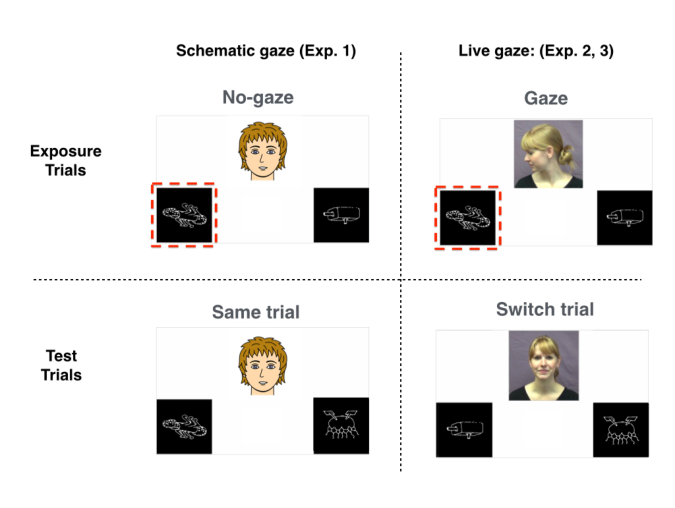
\includegraphics{figs/stimuli-1} \caption[Screenshots of exposure and test trials from Experiment 1 (schematic gaze cue) and Experiments 2 \& 3 (human actress gaze cue)]{Screenshots of exposure and test trials from Experiment 1 (schematic gaze cue) and Experiments 2 \& 3 (human actress gaze cue). Participants saw exposure trials with or without a gaze cue depending on condition assignment. All participants saw both types of test trials: Same and Switch. On Same trials the object that participants chose during exposure appeared with a new novel object. On Switch trials the object that participants did not choose appeared with a new novel object.}\label{fig:stimuli}
\end{figure}
\end{CodeChunk}

\subsubsection{Stimuli}\label{stimuli}

Figure 1 shows screenshots taken from Experiment 1. Visual stimuli were
black and white pictures of familiar and novel objects taken from
Kanwisher, Woods, Iacoboni, \& Mazziotta (1997). Auditory simuli were
recordings of familiar and novel words by an AT\&T Natural Voices
\texttrademark (voice: Crystal) speech synthesizer. Novel words were 1-3
syllable pseudowords that obeyed all rules of English phonotactics. A
schematic drawing of a human speaker was chosen for ease of manipulating
the direction of gaze, the referential cue of interest in this study.
All experiments can be viewed and downloaded at the project page:
\url{https://kemacdonald.github.io/soc_xsit/}.

\subsubsection{Design and Procedure}\label{design-and-procedure}

Participants saw a total of 16 trials: eight exposure trials and eight
test trials. On each trial, they heard one novel word, saw a set of
novel objects, and were asked to guess which object went with the word.
Before seeing exposure and test trials, participants completed four
practice trials with familiar words and objects. These trials
familiarized participants to the task and allowed us to exclude
participants who were unlikely to perform the task as directed either
because of inattention or because their computer audio was turned off.

After the practice trials, participants were told that they would now
hear novel words and see novel objects, and that their task was to
select the referent that ``goes with each word.'' Over the course of the
experiment, participants heard eight novel words two times, with one
exposure trial and one test trial for each word. Four of the test trials
were \emph{Same} trials in which the object that participants selected
on the exposure trial was shown with a set of new novel objects. The
other four test trials were \emph{Switch} trials in which one of the
objects was chosen at random from the set of objects that the
participant did not select on exposure.

Participants were randomly assigned to the 32 between-subjects
conditions (4 Referents X 4 Intervals X 2 Gaze). Participants either saw
2, 4, 6, or 8 referents on the screen and test trials occurred after
either 0, 1, 3, or 7 trials from the initial exposure to a word.
Participants were assigned to the Gaze or No-gaze conditions. In the
Gaze condition, gaze was directed towards one of the objects on exposure
trials; in the No-gaze condition, gaze was always directed straight
ahead (see Figure 1 for examples of these trial types). At test, gaze
was never informative. To show participants that their response had been
recorded, a red box appeared around the selected object for one second.
This box always appeared around the selected object, even if
participants' selections were incorrect.

\subsection{Results and Discussion}\label{results-and-discussion}

\subsubsection{Analysis plan}\label{analysis-plan}

The structure of our analysis plan is parallel across all three
experiments. First, we examine performance on Exposure trials to provide
evidence that learners were (a) sensitive to our experimental
manipulation and (b) altered their allocation of attention in response
to changes in contextual ambiguity. Then we examine performance on Test
trials to show that learners' memory for alternative word-object links
changes depending on the ambiguity of the learning context. The key
behavioral prediction of our hypothesis is that the presence of gaze
will result in reduced memory for multiple word-object links,
operationalized as a decrease in performance on Switch test trials after
seeing Exposure trials with a gaze cue. To quantify participants'
behavior, we use mixed effects regression models with the maximal random
effects structure justified by our experimental design: by-subject
intercepts and slopes for each trial type. All mixed-effects models were
fit using the lme4 package in R (Bates, Maechler, Bolker, \& Walker,
2013), and all of our data, processing, and analysis code can be viewed
in the version control repository for this paper at:
\url{https://github.com/kemacdonald/soc_xsit}.

\begin{CodeChunk}
\begin{figure}[tb]
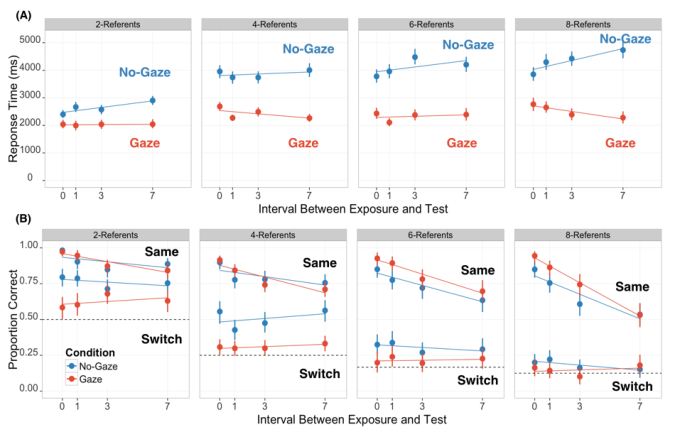
\includegraphics{figs/expt1-plot-1} \caption[Experiment 1 results]{Experiment 1 results. Panel A shows response times on exposure trials across all experimental conditions: Gaze and No-gaze, Referents (2, 4, 6, and 8), and Intervening trials (0, 1, 3, and 7). Panel B shows accuracy on test trials for Same and Switch trials across all conditions. The horizontal dashed lines represent chance performance for each condition. Colored lines are linear model fits and error bars indicate 95\% confidence intervals computed by non-parametric bootstrap.}\label{fig:expt1-plot}
\end{figure}
\end{CodeChunk}

\subsubsection{Exposure trials}\label{exposure-trials}

To ensure that our referential cue manipulation was effective we compare
participant's accuracy
\footnote{Correct performance is defined as selecting the object that was the target of the speaker's gaze.}
on Exposure trials in the Gaze condition to a model of random behavior
defined as a Binomial distribution with a probability of success
\(\frac{1}{Num Referents}\). Following Yurovsky \& Frank (2015), we fit
logistic regressions for each Gaze, Referent, and Interval combination
specified as \texttt{Correct $\sim$ 1 + offset(logit(1/Referents))}. The
offset encodes the chance probability of success given the number of
referents, and the coefficient for the intercept term shows on a
log-odds scale how much more likely participants are to select the gaze
target than would be expected if participants were selecting randomly.
In all conditions participants used gaze to select referents on Exposure
trials more often than expected by chance (smallest \(\beta\) = 2.56, z
= 10.71, p \textless{} .001).

We were also interested in differences in participants' response times
across the experimental conditions. Since these trials were self-paced,
participants could choose how much time to spend studying the referents
on the screen, thus providing an index of participants' attention. To
quantify the effects of gaze, interval, and number of referents, we fit
a linear mixed effects model predicting participants' response times as
follows:
\texttt{RT $\sim$ Gaze Condition * Log(Interval) * Log(Referents) + (1 | subject)}.
We found a significant main effect of referents (\(\beta\) = 806.89, p
\textless{} .001) with slower responses as the number of referents
increased, and a significant two-way interaction between Gaze condition
and number of referents (\(\beta\) = -517.36, p \textless{} .001) such
that responses were faster in the Gaze condition, especially as the
number of referents increased. The interaction between Gaze condition
and number of referents is shown in Panel A of Figure 2. Faster response
times on Exposure trials with gaze provides preliminary evidence that
the presence of a referential cue focused participants' attention on the
gaze target and away from alternative word-object links.

\subsubsection{Test trials}\label{test-trials}

Panel B of Figure 2 shows participants' accuracies in identifying the
referent for each word in all conditions for both kinds of trials (Same
and Switch). We first compared the distribution of correct responses
made by each participant to the distribution expected if participants
were selecting randomly defined as a Binomial distribution with a
probability of success \(\frac{1}{Num Referents}\). We fit the same
logistic regressions as we did for Exposure trials:
\texttt{Correct $\sim$ 1 + offset(logit(1/Referents))}. On 31 out of the
32 conditions for both Same and Switch trials, participants chose the
correct target more often than would be expected by chance (smallest
\(\beta\) = 0.32, z = 1.96, p = 0.05). On Switch trials in the 8
referent, 3 interval condition, participants' responses were not
significantly different from chance (\(\beta\) = 0.09, z = 0.5, p =
0.62). Participants' success on Switch trials replicates the findings
from Yurovsky \& Frank (2015) and provides direct evidence that learners
encoded more than a single hypothesis in ambiguous word learning
situations, even under high attentional and memory demands, and even in
the presence of a referential cue.

\begin{table}[tb]
\centering
\begin{tabular}{lrrrrl}
 Predictor & Estimate & Std. Error & $z$ value & $p$ value &  \\ 
  \hline
Intercept & 2.93 & 0.28 & 10.28 & $<$ .001 & *** \\ 
  Switch Trial & -1.37 & 0.23 & -5.90 & $<$ .001 & *** \\ 
  Gaze Condition & -0.37 & 0.25 & -1.48 & 0.14 &  \\ 
  Log(Interval) & -0.42 & 0.11 & -3.88 & $<$ .001 & *** \\ 
  Log(Referents) & 0.31 & 0.11 & 2.73 & 0.01 & ** \\ 
  Switch Trial*Gaze Condition & -0.81 & 0.12 & -6.77 & $<$ .001 & *** \\ 
  Switch Trial*Log(Interval) & 0.52 & 0.05 & 9.53 & $<$ .001 & *** \\ 
  Switch Trial*Log(Referent) & -0.60 & 0.09 & -6.94 & $<$ .001 & *** \\ 
  Gaze Condition*Log(Interval) & 0.02 & 0.06 & 0.31 & 0.76 &  \\ 
  Gaze Condition*Log(Referent) & 0.26 & 0.09 & 2.79 & 0.01 & ** \\ 
  Log(Interval)*Log(Referent) & -0.06 & 0.04 & -1.42 & 0.15 &  \\ 
   \hline
\end{tabular}
\caption{Predictor estimates with standard errors and significance information for a logistic mixed-effects model predicting word learning in Experiment 1.} 
\label{tab:exp1_reg}
\end{table}

To quantify the effect of each predictor on the probability of a correct
response, we fit the following mixed-effects logistic regression model
to a filtered dataset, removing participants who were not reliably
selecting the referent that was the target of gaze on exposure
trials:\footnote{We did not predict that there would be a subset of participants who would not follow the gaze cue, thus this filtering criteria was developed post-hoc. However, we believe the filter is theoretically motivated because we would only expect to see an effect of gaze if participants were actually using the gaze cue. The filter removes 90 participants who did not reliably select the gaze target on exposure trials. The key inferences from the data do not depend on this filtering criteria.}
\texttt{Correct $\sim$ Trial Type * Gaze + Trial Type * Log(Interval) + Trial Type * Log(Referents) + \\ offset(logit($^1/_{Referents}$)) + (TrialType | subject)}.
We follow Yurovsky \& Frank (2015)'s analysis plan and coded interval
and number of referents as continuous predictors and transformed these
variables to the log scale. We limited the model to include only two-way
interactions because the critical test of our hypothesis is the
interaction between Gaze condition and Trial Type, and we did not have
any theoretical predictions for possible three-way
interactions.\footnote{If we allow for three-way interactions in the model, there is a significant interaction between Gaze condition, Trial Type, and Interval ($\beta = 0.31$, p $<$ .01). The two-way interaction betwen Gaze condition and Trial Type remains significant in this more complex model. A model including four-way interactions did not sufficiently improve model fit in order to justify the added complexity.}

Table 1 shows the output of the logistic regression. We found
significant main effects of Referents (\(\beta = 0.31\), p \textless{}
.001) and Interval (\(\beta = -0.42\), p \textless{} .001), such that as
each of these factors increased, accuracy on test trials decreased. We
also found significant main effects of Trial Type (\(\beta = -1.37\), p
\textless{} .001), with worse overall performance on Switch trials.
There were significant interactions between Trial Type and Interval
(\(\beta = 0.52\), p \textless{} .001), Trial Type and Referents
(\(\beta = -0.6\), p \textless{} .001), and Gaze condition and Referents
(\(\beta = 0.26\), p \textless{} .05). These interactions can be
interpreted as (a) the interval between exposure and test affecting Same
trials more than Switch trials, (b) the number of referents affecting
Switch trials more than Same trials, and (c) participants performing
slightly better at higher number of referents in the Gaze condition (see
Panel B of Figure 2). The interactions between Gaze condition and
Referents and between Referents and Interval were not significant.
Crucially, we found the predicted interaction between Trial Type and
Gaze condition (\(\beta = -0.81\), p \textless{} .001), with
participants in the Gaze condition performing worse on Switch trials.
This interaction provides direct evidence that the presence of a
referential cue selectively reduced participants' memory for alternative
word-object links.

Taken together, the response time and accuracy analyses provide evidence
that the presence of a referential cue modulated learners' attention
during learning, and in turn made them less likely to track multiple
word-object links. We did not see strong evidence that reduced tracking
of alternatives resulted in an increase in performance on Same trials.
This finding suggests that the limitations on Same trials may be
different than those regulating the distribution of attention on Switch
trials, since the presence of a referential cue selectively reduced
learners tracking of alternatives but apparently did not lead learners
to form a stronger memory of their single candidate hypothesis.

There was relatively large variation in performance across conditions in
group-level accuracy scores and in participants' tendency to \emph{use}
the referential cue on exposure trials. Moreover, we found a subset of
participants who did not reliably use the gaze cue at all, potentially
reducing the effect of gaze on cross-situational learning in this
experiment. It is possible that the effect of gaze was reduced because
the referential cue that we used -- a static schematic drawing of a
speaker -- was relatively weak compared to the cues present in real
world learning environments. We do not yet know how learners' memory for
alternatives during cross-situational learning would change in the
presence of a stronger and more ecologically valid referential cue.
Experiment 2 attempts to answer this question.

\section{Experiment 2}\label{experiment-2}

In Experiment 2, we attempt to replicate the findings from Experiment 1
using a more ecologically valid stimulus set. To move closer to a real
world referential cue, we replaced the static, schematic drawing with a
live actress. To reduce the across-conditions variability, we introduced
a within-subjects design where each participant saw both Gaze and
No-gaze exposure trials. We selected a subset of conditions from
Experiment 1, testing only the 4-referent display with 0 and 3
intervening trials as between-subjects manipulations. Our goals were to
replicate the reduction in learners' multiple alternatives tracking in
the presence of referential cues, and to test whether increasing the
ecological validity of the cue would result in a boost to the strength
of learners' recall of their single candidate hypothesis.

\subsection{Method}\label{method-1}

\subsubsection{Participants}\label{participants-1}

Participant recruitment and inclusionary/exclusionary criteria were
identical to those of Experiment 1 (excluded 36 HITs). 100 HITs were
posted for each condition (1 Referent X 2 Intervals X 2 Gaze conditions)
for total of 400 paid HITs.

\subsubsection{Stimuli}\label{stimuli-1}

Audio and picture stimuli were identical to Experiment 1. The
referential cue in the Gaze condition was a video (see Figure 1). On
each exposure trial, the actress looked out at the participant with a
neutral expression, smiled, and then turned to look at one of the four
images on the screen. She maintained her gaze for 3 seconds before
returning to the center. On test trials, she looked straight ahead for
the duration of the trial.

\subsection{Design and Procedure}\label{design-and-procedure-1}

Procedures were identical to those of Experiment 1. The major design
change was a within-subjects manipulation of the gaze cue with each
participant seeing exposure trials with and without gaze. The experiment
consisted of 32 trials broken down into 2 blocks of 16 trials. Each
block consisted of 8 exposure trials and 8 test trials (4 Same trials
and 4 Switch trials), and contained only Gaze or No-gaze exposure
trials. The order of block was counterbalanced across participants.

\subsection{Results and Discussion}\label{results-and-discussion-1}

We followed the same analysis plan as in Experiment 1, first analyzing
performance on exposure trials, and then analyzing performance on test
trials.

\subsubsection{Exposure trials}\label{exposure-trials-1}

Similar to Experiment 1, participants' responses on exposure trials
differed from those expected by chance (smallest \(\beta\) = 3.42, z =
33.43, p \textless{} .001), suggesting that gaze was effective in
directing attention to the target referent. Participants in Experiment 2
were numerically more consistent in their use of gaze with the live
action stimuli compared to the schematic stimuli used in Experiment 1
(\(M_1 = .76, M_2 = .81\)), suggesting that using a live actress
resulted in a slight increase in participants' willingness to follow the
gaze cue.

Panel A of figure 3 shows participants' response times. We replicate the
findings from Experiment 1, with faster response times in Gaze
condition. We fit a linear mixed effects model to response times with
the same specification as Experiment 1, finding main effects for Gaze
condition (\(\beta\) = -1112.83, p \textless{} .001) and Interval
(\(\beta\) = -498.96, p \textless{} .001) with faster responses in the
Gaze condition and in the longer Interval conditions. The two-way
interaction between Gaze condition and interval was not significant,
with gaze having the same effect on participants' response times at both
intervals.

\begin{CodeChunk}
\begin{figure}[tb]
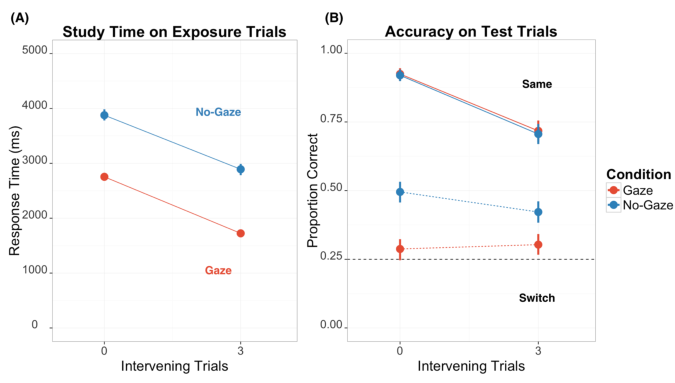
\includegraphics{figs/expt2-plot-1} \caption[Experiment 2 results]{Experiment 2 results. Panel A shows study times for exposure trials with and without gaze. Panel B shows accuracy on test trials for same and Switch trials across all conditions. The dashed line in Panel B represents chance performance. Error bars indicate 95\% confidence intervals computed by non-parametric bootstrap.}\label{fig:expt2-plot}
\end{figure}
\end{CodeChunk}

\subsubsection{Test trials}\label{test-trials-1}

\begin{table}[tb]
\centering
\begin{tabular}{lrrrrl}
 Predictor & Estimate & Std. Error & $z$ value & $p$ value &  \\ 
  \hline
Intercept & 2.69 & 0.16 & 16.84 & $<$ .001 & *** \\ 
  Switch Trial & -2.74 & 0.16 & -17.04 & $<$ .001 & *** \\ 
  Gaze Condition & -0.12 & 0.16 & -0.75 & 0.45 &  \\ 
  Log(Interval) & -0.88 & 0.09 & -9.40 & $<$ .001 & *** \\ 
  Switch Trial*Gaze Condition & -0.73 & 0.15 & -4.85 & $<$ .001 & *** \\ 
  Switch Trial*Log(Interval) & 0.76 & 0.09 & 8.35 & $<$ .001 & *** \\ 
  Gaze Condition*Log(Interval) & 0.13 & 0.07 & 1.81 & 0.07 & . \\ 
   \hline
\end{tabular}
\caption{Predictor estimates with standard errors and significance information for a logistic mixed-effects model predicting word learning in Experiment 2.} 
\label{tab:exp2_reg}
\end{table}

Panel B of Figure 3 shows performance on test trials in Experiment 2.
Across all conditions for both Trial Types participants selected the
correct referent at rates greater than chance (smallest \(\beta\) =
0.55, z = 9.04, p \textless{} .001). We replicate the critical finding
from Experiment 1: after seeing exposure trials with gaze, participants
performed worse on Switch trials, providing evidence that they stored
fewer word-object links. We fit a mixed-effects logistic regression
model with the same specifications as in Experiment 1 and found
significant main effects of Interval (\(\beta = -0.88\), p \textless{}
.001) and Trial Type (\(\beta = -2.74\), p \textless{} .001).
Participants were less accurate as the interval between exposure and
test increased and on the Switch trials overall.

In addition, there was a significant two-way interaction between Trial
Type and Interval (\(\beta = 0.76\), p \textless{} .001), with worse
performance on Switch trials at the higher intervals, and a marginal
two-way interaction betwen Gaze condition and Interval
(\(\beta = 0.13\), p = 0.07) such that the number of intervening trials
had a smaller effect on participants' performance in the Gaze condition.
We found a robust interaction between Gaze condition and Trial Type
(\(\beta = -0.73\), p \textless{} .001) with Switch trials being more
difficult after gaze exposure
trials.\footnote{As in Experiment 1, we fit this model a filtered dataset removing participants who did not reliably use the gaze cue.}
Once again, we did not see evidence of a boost to performance on Same
trials in the Gaze condition.

The results of Experiment 2 provide converging evidence for our
hypothesis, showing that the presence of a referential cue reliably
focused learners' attention away from alternative word-object links and
shifted them towards single hypothesis tracking. Changing to a live
action stimulus set led to slightly higher rates of selecting the target
of gaze on exposure trials, but did not result in a boost to performance
on Same trials. The selective effect of gaze on Switch trials provides
additional evidence that the fidelity of participants' single hypothesis
was unaffected by the presence of a referential cue in our paradigm.

Thus far we have shown that people store different amounts of
information in response to a categorical manipulation of referential
uncertainty. In both Experiments 1 and 2, the learning context was
either entirely ambiguous (No-gaze) or entirely unambiguous (Gaze). But
not all real world learning contexts fall at the extremes of this
continuum (although see Yurovsky et al., 2013). Could learners be
sensitive to more subtle changes in the quality of learning contexts? In
our next experiment, we test a clear prediction of our account: whether
learners tendency to store multiple word-object links responds to graded
changes of referential uncertainty during learning.

\section{Experiment 3}\label{experiment-3}

In Experiment 3, we explore whether learners will allocate attention and
memory flexibly in response to \emph{graded} changes in the referential
uncertainty present during learning. To test this hypothesis, we move
beyond a categorical manipulation of the presence/absence of gaze, and
we parametically vary the strength of the referential cue. We manipulate
cue strength by including a block of familiarization trials at the start
of the experiment where we establish the reliability of the speaker's
gaze. This design was inspired by a growing body of experimental work
showing that even young children are sensitive to the prior reliability
of speakers and will use this information when deciding whom to learn
novel words from (Koenig, Clement, \& Harris, 2004).

\subsection{Method}\label{method-2}

\subsubsection{Participants}\label{participants-2}

Participant recruitment, and inclusionary/exclusionary criteria were
identical to those of Experiment 1 and 2 (excluded 4 HITs). 100 HITs
were posted for each reliability level (0\%, 25\%, 50\%, 75\%, and
100\%) for total of 500 paid HITs.

\subsubsection{Design and Procedure}\label{design-and-procedure-2}

Procedures were identical to those of Experiment 1 and 2. We modified
our cross-situational learning paradigm to include a block of 16
familiarization trials (8 exposure trials and 8 test trials), which
established the reliability of the speaker. To establish reliability, we
varied the proportion of Same/Switch trials that occurred during this
familiarization block. Recall that on Switch trials the gaze target does
not show up at test, thus providing evidence that this speaker's gaze
might not be a reliable cue to reference. Gaze reliability was a
between-subjects manipulation, with participants either seeing 0, 2, 4,
6, or 8 Switch trials. After the familiarization block, participants
completed another block of 16 trials (8 exposure trials and 8 test
trials). Since we were no longer testing the effect of the presence or
absence of a referential cue, all exposure trials in Experiment 3
included gaze, but this cue was more or less reliable depending on which
familiarization block participants saw. Finally, at the end of the task
we asked participants to assess the reliability of the speaker on a
continuous scale from ``completely unreliable'' to ``completely
reliable.''

\subsection{Results and Discussion}\label{results-and-discussion-2}

\subsubsection{Exposure trials}\label{exposure-trials-2}

Similar to Experiments 1 and 2, participants reliably chose the referent
that was the target of gaze at rates greater than those that would be
predicted by a guessing model (smallest \(\beta\) = 2.57, z = 33.43, p
\textless{} .001). To quantify the effect of reliability condition and
particpants' subjective reliablity assessment, we fit a mixed effects
logistic regression model predicting the probability of selecting the
gaze target as follows:
\texttt{Correct-Exposure $\sim$ Reliability Condition * Subjective Reliability + offset(logit(1/Referents)) + (1 | subject)}.
We found significant main effects of both reliability condition
(\(\beta\) = 3.3, p \textless{} .05) and subjective reliabilty
(\(\beta\) = 7, p \textless{} .001) such that when the gaze cue was more
reliable and when subjective reliability assessments were higher
participants were more likely to use the gaze cue. The interaction
between speaker reliability and subjective reliablity assessments was
marginally significant (\(\beta\) = -4.33, p = 0.1). This analysis
provides evidence that participants were sensitive to the reliability
manipulation both in how often they used the gaze cue during the task
and in how they rated the speaker at the end of the task.

\begin{CodeChunk}
\begin{figure}[tb]
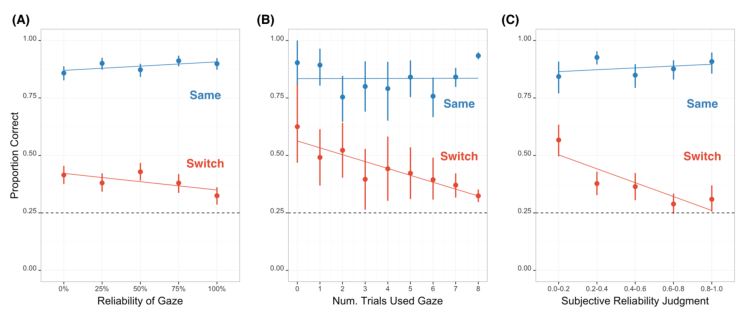
\includegraphics{figs/expt3-plot-1} \caption[Accuracy on test trials in Experiment 3 for both same and switch trial types]{Accuracy on test trials in Experiment 3 for both same and switch trial types. Panel A shows accuracy as a function of the speaker's reliability. Panel B shows accuracy as a function of participants' gaze following on exposure trials. Panel C shows accuracy as a function of participants' subjective reliability judgments, grouped into five equally spaced bins. The horizontal dashed line represents the expected performance if participants were selecting randomly. The colored lines are linear model fits and error bars indicate 95\% confidence intervals computed by non-parametric bootstrap.}\label{fig:expt3-plot}
\end{figure}
\end{CodeChunk}

\subsubsection{Test trials}\label{test-trials-2}

Figure 4 shows performance on test trials in Experiment 3. Across all
conditions for both Trial Types participants selected the correct
referent at rates greater than chance (smallest \(\beta\) = 0.41, z =
3.63, p \textless{} .001). Our primary prediction in this experiment is
an interaction between reliability and test trial type, with higher
levels of reliability leading to less attention and memory allocated to
alternative word-object links. To test this prediction, we performed
three complementary analyses of test trial performance using three
different predictors: reliability condition, participants' use of gaze,
and participants' subjective reliablity assessment.

\paragraph{Reliability condition
analysis}\label{reliability-condition-analysis}

Panel A of Figure 4 shows participants' accuracy on both types of test
trials as a function of the reliablity manipulation. We fit a
mixed-effects logistic regression model predicting accuracy using
reliability condition as a predictor and found a significant main effect
of trial type (\(\beta = -1.85\), p \textless{} .001), with lower
accuracy on Switch trials. We found a significant interaction between
Reliability condition and Trial Type (\(\beta = -0.9\), p = 0.05),
providing evidence for our key prediction. The interaction between
Reliability condition and accuracy was relatively weak, however, and --
similar to Experiment 1 -- there was substantial variability across
conditions (see the 50\% reliable condition in Panel A of Figure 4). To
provide additional support for our hypothesis, we conducted two
follow-up analyses.

\paragraph{Gaze use analysis}\label{gaze-use-analysis}

We would only expect to see a strong interaction between reliability and
trial type if learners chose to use the gaze cue during exposure trials.
To test this hypothesis, we fit a mixed effects logistic regression
model with the same specifications, but substituting accuracy on
exposure trials for reliability condition as a predictor. We found a
robust two-way interaction between accuracy on exposure trials and Trial
Type (\(\beta = -0.36\), p \textless{} .001) such that participants who
were more likely to use the gaze cue performed worse on Switch trials,
but not Same trials.\footnote{We found this interaction while performing
  exploratory data analysis on a previous version of this study with an
  independent sample (N = 250, \(\beta = -0.28\), p \textless{} .001).
  The results reported here are from a follow-up study where testing
  this interaction was a planned analysis.} Panel B of Figure 4 shows
this interaction.

\paragraph{Subjective reliability
analysis}\label{subjective-reliability-analysis}

The strong interaction between frequency of gaze use and test trial
performance suggests that participants' subjective experience of
reliablity in the experiment mattered. To quantify the effect of
subjective reliablity, we fit the same mixed effects logistic regression
model, but substituted subjective reliability as a predictor of test
trial performance. We found a signficant interaction between Trial Type
and participants' subjective reliability assessements
(\(\beta = -1.37\), p = 0.02) -- if participants thought the speaker was
more reliable, then they performed worse on Switch, but not Same,
trials.

Taken together, these three analyses show that as the speaker's gaze
became more reliable, participants were (a) more likely to use it, (b)
more likely to rate the speaker as reliable, and (c) less likely to
store multiple word-object links. These findings support and extend the
results of Experiments 1 and 2 in several important ways. First,
participants' performance on Same trials was again relatively unaffected
by changes in peformance on Switch trials. The selective effect of gaze
on Switch trials provides converging evidence that the limitations on
Same trials may be different than those regulating the distribution of
attention on Switch trials. Second, learners' \emph{use} of a
referential cue was a stronger predictor of reduced memory for
alternative word-object links compared to our reliablity manipulation.
Although we found a significant effect of reliability on participants'
use of the gaze cue, participants' tendency to use the cue remained
high. Consider that even in the 0\% reliability condition the mean
proportion of gaze following was still 0.82. It is reasonable that
participants would continue to use the gaze cue in our experiment since
it was the only cue available and participants did not have a strong
reason to think that the speaker would be deceptive.

The critical contribution of Experiment 3 is the finding that learners
respond to a \emph{graded} manipulation of referential uncertainty, with
the amount of information stored from the intital exposure tracking with
both the reliability of the cue and participants' use of the cue. This
graded accuracy performance provides support for a critical prediction
of our account: that learners store a single candidate word meaning and
a set of alternatives with different levels of fidelity depending on the
amount of referential uncertainty present during learning.

\section{General Discussion}\label{general-discussion}

Tracking cross-situational word-object statistics allows word learning
to proceed despite the presence of individually ambiguous naming events.
But models of cross-situational learning disagree about how much
information is actually stored in memory and how to best characterize
the input to statistial learning mechanisms. In the current line of
work, we explore the hypothesis that these two factors are fundamentally
linked, both to one another and to the social context in which word
learning occurs. Specifically, we ask how cross-situational learning
operates over social input that varies along a continuum from low to
high ambiguity.

Our results suggest that the representations underlying
cross-situational learning are quite flexible. In the absence of a
referential cue to word meaning, learners were more likely to store
alternative word-object links. In contrast, when gaze was present, they
stored less information, showing behavior consistent with tracking a
single hypothesis (Experiments 1 and 2). Learners were also sensitive to
a parametric manipulation of the referential cue, showing a graded
increase in the tendency to use the cue as reliability increased, which
in turn resulted in a graded decrease in memory for alternative
word-object links (Experiment 3). Across all three experiments, reduced
memory for alternative hypotheses did not result in a boost in memory
for learners' candidate hypothesis. This pattern of data suggests that
the presence of a referential cue selectively affected one component of
the underlying representation: the number of alternative word-object
links, and not learners candidate hypothesis.

Why did we not see an increase in the strength of learners' candidate
hypothesis? One possibility is that participants did not shift their
cognitive resources from the set of alternatives to their single
hypothesis, but instead rationally conserved their resources for future
use. Griffiths, Lieder, \& Goodman (2015) formalize this behavior by
pushing the rationality of computational-level models down to the
psychological process level. In their framework, cognitive systems are
thought to be adaptive in that they optimize the use of their limited
resources, taking the cost of computation (e.g., opportunity cost of
time or mental opportunity) into account. For example, Vul, Goodman,
Griffiths, \& Tenenbaum (2014) showed that as time pressure increased in
a decision-making task, participants were more likely to show behavior
consistent with a less cognitively challenging strategy of matching,
rather than with the globally optimal strategy. Here, we show evidence
that learners adapt their allocation of cognitive resources to the level
of referential uncertainty in the learning context, spending less time
studying alternative word-object links and reducing the number of links
stored in memory when uncertainty is low.

Our results also fit well with recent experimental work that
investigates how attention and memory can constrain infants' statistical
word learning. For example, L. B. Smith \& Yu (2013) used a modified
cross-situational learning task to show that only infants who disengaged
from a novel object to look at both potential referents were able to
learn the correct word--object mappings. Moreover, Vlach \& Johnson
(2013) showed that 16-month-olds were only able to learn from adjacent
cross-situational co-occurrence statistics, and unable to learn from
co-occurrences that were separated in time. Both of these findings make
the important point that only the data that comes into contact with the
learning system can be used for cross-situational word learning, and
this data is directly influenced by the attention and memory constraints
of the learner. Our findings suggest that referential cues could play an
important role in constraining the input to statistical learning
mechansims.

How should we characterize the effect of social information on attention
and memory in our task? One possibility is that the referential cue acts
as a filter, only allowing likely referents to contact statistical
learning mechansims (Yu \& Ballard, 2007). This `filtering account'
separates the effect of social cues from the underlying computation that
aggregates cross-situational information. Another possibility is that
referential cues provide evidence about a speaker's communicative intent
(Frank, Goodman, \& Tenenbaum, 2009). In this model, the learner is
reasoning about the speaker and word meanings simultaneously, which
places inferences based on social information as part of the underlying
computation. A third possibility is that participants thought of the
referential cue as pedagogical. In this scenario, learners assume that
the speaker will choose an action that is most likely to increase the
learner's belief in the true state of the world (Shafto, Goodman, \&
Frank, 2012), making it unnecessary to allocate resources to alternative
hypotheses. Experiments show that children spend less time exploring an
object and are less likely to discover alternative object-functions, if
a single function is demonstrated in a pedagogical context (Bonawitz et
al., 2011). However, because the results from the current study cannot
distinguish between these explanations, these questions remain topics
for future studies specifically designed to tease apart these
possibilities.

There are several limitations to the current study that are worth
noting. First, the social context we used was relatively impoverished.
Although we moved beyond a simple manipulation of the presence or
absence of social information, we isolated just a single cue to
reference, gaze. But real-world learning contexts are much more complex,
providing learners access to multiple cues such as gaze, pointing, and
previous discourse. In fact, Frank, Tenenbaum, \& Fernald (2013)
analyzed a corpus of parent-child interactions and concluded that
learners would do better to aggregate noisy social information from
multiple cues, rather than monitor a single cue, because no single cue
was a consistent predictor of reference in their corpus. In our data, we
did see a more reliable effect of referential cues when we used a live
actress, which included both gaze and head turn as opposed to the
static, schematic stimuli, which only included gaze. It is still an open
and interesting question as to how our results would generalize to
real-world learning environments that contain a rich combination of
social cues.

Second, we do not yet know how these results would generalize to young
word learners. Research with infants' shows rapid development of visual
attention and memory in the first years of life (Colombo, 2001;
Ross-sheehy, Oakes, \& Luck, 2003). Moreover, experimental work shows
that infants' attention is often stimulus driven and sticky (Oakes,
2011), suggesting that very young word learners might not effectively
explore the visual scene to extract the necessary statistics for
effective cross-situational word learning. The current work suggests
that referential cues might play an even more important role for young
learners, guiding them to the relevant statistics in the input.

And third, in the current experiments we tested a minimal
cross-situational learning scenario. Our task contained only one
exposure for each novel word-object pairing. In contrast, real world
naming events are best characterized by discourse, where an object is
likely to be named repeatedly in a short amount of time (Frank et al.,
2013; Rohde \& Frank, 2014). Moreover, we presented novel words in
isolation, removing any sentential cues to word meaning (e.g.,
verb-argument relations). Previous work shows that sentence-level
constraints do interact with cross-situational word learning mechansims
(Koehne \& Crocker, 2014). We need more evidence to understand how
representations underlying cross-situational learning change in response
to referential uncertainty at different timescales and in richer
language contexts that more accurately reflect learning environments.

Word learning proceeds despite the potential for high levels of
referential uncertainty and learners' limited cognitive resources. Our
work shows that cross-situational learners flexibly respond to the
amount of ambiguity in the input, and as referential uncertainty
increases, learners store more word-object links. Overall, these results
bring together aspects of both social and statistical accounts of word
learning, and increase our understanding of how statistical learning
mechanisms operate over fundamentally social input.

\newpage

\section*{References}\label{references}
\addcontentsline{toc}{section}{References}

Baldwin, D. A. (1993). Infants' ability to consult the speaker for clues
to word reference. \emph{Journal of Child Language}, \emph{20}(02),
395--418.

Bates, D., Maechler, M., Bolker, B., \& Walker, S. (2013). Lme4: Linear
mixed-effects models using eigen and s4. \emph{R Package Version},
\emph{1}(4).

Bloom, P. (2002). \emph{How children learn the meaning of words}. The
MIT Press.

Bonawitz, E., Shafto, P., Gweon, H., Goodman, N. D., Spelke, E., \&
Schulz, L. (2011). The double-edged sword of pedagogy: Instruction
limits spontaneous exploration and discovery. \emph{Cognition},
\emph{120}(3), 322--330.

Brooks, R., \& Meltzoff, A. N. (2005). The development of gaze following
and its relation to language. \emph{Developmental Science}, \emph{8}(6),
535--543.

Brooks, R., \& Meltzoff, A. N. (2008). Infant gaze following and
pointing predict accelerated vocabulary growth through two years of age:
A longitudinal, growth curve modeling study. \emph{Journal of Child
Language}, \emph{35}(01), 207--220.

Carpenter, M., Nagell, K., Tomasello, M., Butterworth, G., \& Moore, C.
(1998). Social cognition, joint attention, and communicative competence
from 9 to 15 months of age. \emph{Monographs of the Society for Research
in Child Development}, i--174.

Cartmill, E. A., Armstrong, B. F., Gleitman, L. R., Goldin-Meadow, S.,
Medina, T. N., \& Trueswell, J. C. (2013). Quality of early parent input
predicts child vocabulary 3 years later. \emph{Proceedings of the
National Academy of Sciences}, \emph{110}(28), 11278--11283.

Clark, E. V. (2009). \emph{First language acquisition}. Cambridge
University Press.

Cleveland, A., Schug, M., \& Striano, T. (2007). Joint attention and
object learning in 5-and 7-month-old infants. \emph{Infant and Child
Development}, \emph{16}(3), 295--306.

Colombo, J. (2001). The development of visual attention in infancy.
\emph{Annual Review of Psychology}, \emph{52}(1), 337--367.

Frank, M. C., Goodman, N. D., \& Tenenbaum, J. B. (2009). Using
speakers' referential intentions to model early cross-situational word
learning. \emph{Psychological Science}, \emph{20}(5), 578--585.

Frank, M. C., Tenenbaum, J. B., \& Fernald, A. (2013). Social and
discourse contributions to the determination of reference in
cross-situational word learning. \emph{Language Learning and
Development}, \emph{9}(1), 1--24.

Griffiths, T. L., Lieder, F., \& Goodman, N. D. (2015). Rational use of
cognitive resources: Levels of analysis between the computational and
the algorithmic. \emph{Topics in Cognitive Science}, \emph{7}(2),
217--229.

Hollich, G. J., Hirsh-Pasek, K., Golinkoff, R. M., Brand, R. J., Brown,
E., Chung, H. L., \ldots{} Bloom, L. (2000). Breaking the language
barrier: An emergentist coalition model for the origins of word
learning. \emph{Monographs of the Society for Research in Child
Development}, i--135.

Kanwisher, N., Woods, R. P., Iacoboni, M., \& Mazziotta, J. C. (1997). A
locus in human extrastriate cortex for visual shape analysis.
\emph{Journal of Cognitive Neuroscience}, \emph{9}(1), 133--142.

Koehne, J., \& Crocker, M. W. (2014). The interplay of cross-situational
word learning and sentence-level constraints. \emph{Cognitive Science}.

Koenig, M. A., Clement, F., \& Harris, P. L. (2004). Trust in testimony:
Children's use of true and false statements. \emph{Psychological
Science}, \emph{15}(10), 694--698.

McMurray, B., Horst, J. S., \& Samuelson, L. K. (2012). Word learning
emerges from the interaction of online referent selection and slow
associative learning. \emph{Psychological Review}, \emph{119}(4), 831.

Medina, T. N., Snedeker, J., Trueswell, J. C., \& Gleitman, L. R.
(2011). How words can and cannot be learned by observation.
\emph{Proceedings of the National Academy of Sciences}, \emph{108}(22),
9014--9019.

Oakes, L. M. (2011). \emph{Infant perception and cognition: Recent
advances, emerging theories, and future directions}. Oxford University
Press, USA.

Quine, W. V. (1960). 0. word and object. \emph{111e MIT Press}.

Rohde, H., \& Frank, M. C. (2014). Markers of topical discourse in
child-directed speech. \emph{Cognitive Science}, \emph{38}(8),
1634--1661.

Ross-sheehy, S., Oakes, L. M., \& Luck, S. J. (2003). The development of
visual short-term memory capacity in infants. \emph{Child Development},
\emph{74}(6), 1807--1822.

Shafto, P., Goodman, N. D., \& Frank, M. C. (2012). Learning from others
the consequences of psychological reasoning for human learning.
\emph{Perspectives on Psychological Science}, \emph{7}(4), 341--351.

Siskind, J. M. (1996). A computational study of cross-situational
techniques for learning word-to-meaning mappings. \emph{Cognition},
\emph{61}(1), 39--91.

Smith, K., Smith, A. D., \& Blythe, R. A. (2011). Cross-situational
learning: An experimental study of word-learning mechanisms.
\emph{Cognitive Science}, \emph{35}(3), 480--498.

Smith, L. B., \& Yu, C. (2013). Visual attention is not enough:
Individual differences in statistical word-referent learning in infants.
\emph{Language Learning and Development}, \emph{9}(1), 25--49.

Smith, L. B., Suanda, S. H., \& Yu, C. (2014). The unrealized promise of
infant statistical word--referent learning. \emph{Trends in Cognitive
Sciences}, \emph{18}(5), 251--258.

Smith, L., \& Yu, C. (2008). Infants rapidly learn word-referent
mappings via cross-situational statistics. \emph{Cognition},
\emph{106}(3), 1558--1568.

Trueswell, J. C., Medina, T. N., Hafri, A., \& Gleitman, L. R. (2013).
Propose but verify: Fast mapping meets cross-situational word learning.
\emph{Cognitive Psychology}, \emph{66}(1), 126--156.

Vlach, H. A., \& Johnson, S. P. (2013). Memory constraints on infants'
cross-situational statistical learning. \emph{Cognition}, \emph{127}(3),
375--382.

Vouloumanos, A. (2008). Fine-grained sensitivity to statistical
information in adult word learning. \emph{Cognition}, \emph{107}(2),
729--742.

Vul, E., Goodman, N., Griffiths, T. L., \& Tenenbaum, J. B. (2014). One
and done? Optimal decisions from very few samples. \emph{Cognitive
Science}, \emph{38}(4), 599--637.

Wu, R., Gopnik, A., Richardson, D. C., \& Kirkham, N. Z. (2011). Infants
learn about objects from statistics and people. \emph{Developmental
Psychology}, \emph{47}(5), 1220.

Yoon, J. M., Johnson, M. H., \& Csibra, G. (2008). Communication-induced
memory biases in preverbal infants. \emph{Proceedings of the National
Academy of Sciences}, \emph{105}(36), 13690--13695.

Yu, C., \& Ballard, D. H. (2007). A unified model of early word
learning: Integrating statistical and social cues.
\emph{Neurocomputing}, \emph{70}(13), 2149--2165.

Yu, C., \& Smith, L. B. (2007). Rapid word learning under uncertainty
via cross-situational statistics. \emph{Psychological Science},
\emph{18}(5), 414--420.

Yu, C., \& Smith, L. B. (2012). Embodied attention and word learning by
toddlers. \emph{Cognition}.

Yurovsky, D., \& Frank, M. C. (2015). An integrative account of
constraints on cross-situational learning. \emph{Cognition}.

Yurovsky, D., Smith, L. B., \& Yu, C. (2013). Statistical word learning
at scale: The baby's view is better. \emph{Developmental Science},
\emph{16}(6), 959--966.

\bibliography{}

\end{document}
